\section{Background estimation}

In this analysis, the background estimation in the signal regions is
obtained by fitting the (generally multi-dimensional) spectrum of
dimuon masses in data to a sum of signal and background templates with
either both signal and background normalizations floating (for the topology
with exacty one dimuon) or the signal normalization floating and the 
background normalization constrained in the off-diagonal side-band region 
of multi-dimensional distribution of dimuon invariant masses. Modeling of the signal shape is
discussed in Sec.~\ref{sec:signal_mass_spectrum_shape}, and the shapes
of the distributions for backgrounds are modeled by using
appropriately selected background-enriched samples, described below.

Because signal regions are expected to have near-zero background
contamination, our final results only weakly depend on possible
imperfections in modeling the background shape predictions. However,
interpretation of a possible discovery motivated us to perform a thorough
study of the dimuon mass distributions and careful consideration in
constructing the background templates used in the fit. The shape
templates for background mass distributions are derived from
background-enriched samples, in which Standard Model sources dominate
over any potential signals.  These samples must have the same Standard
Model physics content as the corresponding signal regions, which requires
a thorough understanding of the background data. We validate our
techniques and check for possible biases using data in suitably
defined control regions, still dominated by Standard Model
sources, but closer to the signal in event kinematics.

\subsection{Features of low-mass dimuon spectrum}
\label{sec:lowmassspectrum}

To investigate the features of the low-mass single-dimuon spectrum
($0.25<m_{\mu\mu}<5$ GeV/$c^2$), we use events in data satisfying
minimal acceptance requirements and trigger selections (described in
Sec.~\ref{sec:acceptance}). To avoid unblinding any of the signal
regions, we require events to have no additional analysis-quality muon
candidates ($p_T>5$ GeV/$c$ and $|\eta|<2.4$), and the transverse
momentum of the dimuon must be less than 80~GeV/$c$.

The selected region contains events from several Standard Model
processes. The largest contribution is from QCD multi-jet production,
including $J/\psi$, $\psi'$, $\phi$, $\rho/\omega$, and $\eta$ (decays
to $\mu \mu \gamma$) resonances from both light- and heavy-flavor
hadronization, double-semileptonic decay chains from $b$-flavored
hadrons, as well as events with kaon and pion decays-in-flight and
various types of misidentified muons. The second source is prompt
production of the resonances, followed by low-mass Drell-Yan.

To simulate these Standard Model processes, we use the following Monte Carlo samples:
\begin{itemize}
\item inclusive-muon sample skimmed off the Pythia 6 QCD $2\to2$ sample that has $\hat{p}_T > 30$~GeV/$c$, which we divide into three exclusive partitions:
\begin{itemize}
\item $b\bar{b}$ with one $b$-quark decaying to $\mu\mu X$ by double-semileptonic decay or dimuon resonances (both muons have the same $b$-flavored hadron as a common ancestor in the generator-level decay tree);
\item muons from light-flavor hadronization and muons that are unassociated with one another, excluding misidentified muons and decays-in-flight;
\item dimuons with at least one misidentified muon and/or decay-in-flight of a charged pion, charged kaon, or strange baryon;
\end{itemize}
\item prompt $J/\psi \to \mu\mu$, $\psi' \to \mu\mu$, and $\psi' \to J/\psi \, \pi\pi \to \mu\mu \, \pi\pi$, produced with Pythia 6,  decayed with EvtGen (including final state QED radiation);
\item Drell-Yan, generated using Pythia 8 including pile-up (with no explicit low-mass cut-off except that used internally by Pythia).
\end{itemize}

Figure~\ref{fig:support_mass}(a) shows a ``raw'' mass spectrum
overlaid with the ``out-of-the-box'' Monte Carlo predictions using the above
samples, scaled to the integrated luminosity of the dataset
(35~pb$^{-1}$). While there is an excellent general agreement, one can
note several features associated with known deficiencies in
generating the MC samples, e.g.\ the QCD multi-jet sample is missing
$\omega$ and $\psi'$ resonances, and the prompt/Drell-Yan MCs are missing
the $\omega$. Because this analysis will use templates obtained by
fitting actual data distributions, these deficiencies are not a
concern as long as the origin of the discrepancies is 
understood. In addition, there is an excess near the low-mass edge of
the spectrum not explained by the MC.

We undertake additional studies to further our confidence in
understanding the sample composition. This can be important if the
relative fractions of the components present in the low-mass dimuon
spectrum depend strongly on the selections used in the analysis. We first 
divide the data into two subsamples
enriched with $b\bar{b}$ and non-$b\bar{b}$ contributions, respectively. We use
absolute track isolation $Iso$ and transverse vertex displacement
$L_{xy}$ (see
Appendix~\ref{sec:analysis_of_the_low_mass_background_composition} for
definitions) to define the following ``$b\bar{b}$ cuts,''
\begin{equation}
b\bar{b}\mbox{-like {\bf if} (} Iso > 4.5\mbox{ GeV/$c$ {\bf or }} L_{xy} > \mbox{2 mm),}
\label{eqn:bbcuts}
\end{equation}
and we also define the ``anti-$b\bar{b}$ cuts''by inverting this requirement.

The invariant mass distributions for the $b\bar{b}$-enriched and the
$b\bar{b}$-depleted sub-samples is shown in
Figs.~\ref{fig:support_mass}(b) and (c). The comparison affirms our
observation that the inclusive-muon sample simulation is missing
$\omega$ and $\psi'$ resonances, while the prompt/Drell-Yan is missing
the $\omega$. Note that most of the dimuons arising from misidentified
muons and decays-in-flight pass the $b\bar{b}$ cut as these are
typically produced inside jets and therefore are not well
isolated. The fraction of these events comprises about 25\% of the
events with $m_{\mu \mu}<1$~GeV/$c^2$.  Below 0.5~GeV/$c^2$, there is
a low-mass rise not described by the Monte Carlo, and this
distribution is too wide to be a detector resolution-dominated
$\mu\mu$ resonance. This is discussed in further detail in Appendix~\ref{sec:analysis_of_the_low_mass_background_composition} where 
it is shown that a large fraction of these events is due to the not simulated very 
low mass Drell-Yan with the topology of two very close and nearly parallel muon tracks 
causing a poorly measured secondary vertex position and leading to $L_{xy}$
large enough to pass the ``$b\bar{b}$'' selections.

\begin{figure}
\begin{center}
\includegraphics[width=0.45\linewidth]{PLOTS/support_mass_all_logy.pdf}

\includegraphics[width=0.45\linewidth]{PLOTS/support_mass_bbbar_logy.pdf}
\includegraphics[width=0.45\linewidth]{PLOTS/support_mass_antibbbar_logy.pdf}
\end{center}

\caption{ (a): Mass distribution of single-dimuon events with Monte Carlo
  simulations superimposed. (b) and (c): The same distribution for the samples 
enriched with $b\bar{b}$ events (b) and depleted of $b\bar{b}$ events (c). \label{fig:support_mass}}
\end{figure}

\subsection{Background Mass Spectrum in Region (a-1): High-$p_T$ Dimuons}

The (a-1) signal region is defined as exactly one dimuon with the
transverse momentum $p_T^{\mu\mu} > 80$~GeV/$c$. For sufficiently high
$p_T^{\mu\mu}$ (away from threshold effects), the composition of the
Standard Model backgrounds, and therefore the invariant mass
distribution of the single-dimuon sample, is weakly dependent on
$p_T^{\mu\mu}$. To show that the composition of the samples does not
change substantially, Fig.~\ref{fig:support_bbbarcut_limits} compares
the $p_T^{\mu\mu}$ distribution for three sub-classes of single-dimuon
events: (i) non-$J/\psi$ events passing the $b\bar{b}$ cuts, (ii)
$J/\psi$ events passing the $b\bar{b}$ cuts, and (iii) events failing
the $b\bar{b}$ cuts. $J/\psi$ events are selected with a
0.15~GeV/$c^2$-wide mass window around the PDG $J/\psi$ mass. For
$p_T^{\mu\mu}>40$ GeV/c, all three distributions are exponential with
mutually consistent decay length scales.  To show that the shape of
the distribution is weakly dependent on $p_T^{\mu\mu}$,
Fig.~\ref{fig:support_bbbarcut_limits}(b) shows the inclusive-muon MC
mass distributions in 20~GeV/$c$ bins of $p_T^{\mu\mu}$ from 40 to
120~GeV/$c$. We conclude that the mass spectrum of the
background events is negligibly dependent on $p_T^{\mu\mu}$.

Based on the above observations, the (a-1) background template is
obtained by fitting the dimuon invariant mass distribution using
events with $40 < p_T^{\mu\mu} < 60$~GeV/$c$ (the background-enriched
sample). We additionally define a control region, $60 < p_T^{\mu\mu} <
80$~GeV/$c$ for validation.

\begin{figure}
\includegraphics[width=0.50\linewidth]{PLOTS/support_bbbarcut_limits.pdf}
\includegraphics[width=0.50\linewidth]{PLOTS/support_mass_vs_pt.pdf}
\caption{Scaling of single-dimuon data with $p_T$.  Left: $p_T$
  spectra for three non-overlapping subsamples of dimuons ($\propto
  \exp(-x/k)$, normalized by $A$, the integral from 40 to 80~GeV/$c$).
  Right: Mass distribution of inclusive-muon MC in bins of $p_T$ from
  40 to 120~GeV/$c$.  \label{fig:support_bbbarcut_limits}}
\end{figure}

The template shape is obtained by fitting the mass distribution in the background-enriched region to a parametric
function using an unbinned likelihood fit. For uniformity, we use the same function for this and all other background template fits, although we reduce the number of fit parameters when warranted.
\begin{multline}
BG(m;\, p_\omega,\, p_\phi,\, p_{J/\psi},\, p_{\psi'},\, \alpha_{J/\psi},\, \sigma_{J/\psi},\, p_{1/m^2},\, p_{poly},\, p_1,\, ...\,,\, p_n) = \\
p_\omega \, G(m; 0.78265, 0.011) + p_\phi \, G(m; 1.019455, 0.014) + \\
p_{J/\psi} \, CB(m; 3.096916, \sigma_{J/\psi}, \alpha_{J/\psi}) + p_{\psi'} \, G(m; 3.68609, 0.029) + \\
p_{1/m^2} \, 1/m^2 \, ( \int_{0.25}^{5.0}{1/m^2\, dm} )^{-1} + p_{poly} \, B(m; p_1, ..., p_n),
\label{eqn:bkg_shape}
\end{multline}
where $\omega$, $\phi$, and $\psi'$ resonances are parameterized using
$G(m; m_0, \sigma)$, a Gaussian normalized to a unit integral in the
region $0.25 < m < 5$ GeV/c$^2$. For each, $m_0$ is fixed to the
corresponding PDG mass and $\sigma$ (resolution) is fixed to the
resolution obtained in Sec.~\ref{sec:signal_mass_spectrum_shape}. The
$J/\psi$ resonance shape is parameterized with a Crystall Ball
function $CB(m; m_0=3.096916, \sigma_{J/\psi}, \alpha_{J/\psi})$,
normalized to unit area in $0.25 < m < 5$ GeV/c$^2$.  The
$\sigma_{J/\psi}$ and $\alpha_{J/\psi}$ parameters are allowed to
float in fits. The bulk shape is described using $B(m; p_1, ...,
p_n)$, a series expansion in the Bernstein polynomial basis\footnote{E.g.,
  see
  http://www.idav.ucdavis.edu/education/CAGDNotes/Bernstein-Polynomials.pdf. Bernstein
  basis polynomials are positive-definite, thus, by providing $n$
  non-negative coefficients we can get a well behaving
  p.d.f. approximation. We use RooFit's implementation for Bernstein
  basis polynomials.} of degree $n$. The $1/m^2$ term describes the
low-mass Drell-Yan. The $p_\omega$,$p_\phi$, $p_{J/\psi}$, $p_{\psi'}$,
$p_{B}$, and $p_{1/m^2}$ parameters are normalization factors for the
resonances, bulk and the $1/m^2$ components, respectively, and are
obtained from the fit.

Figure~\ref{fig:backgroundEnriched_highpt}(a) shows the background
template obtained by fitting the data from the background-enriched
region. The band indicates the spread in the fitted shape due to
variations of fitted parameters within the measured values. To verify
our assumption that the shape of the backgrounds is not changing
substantially with $p_T^{\mu\mu}$,
Fig.~\ref{fig:backgroundEnriched_highpt}(b) shows the same template
overlaid with the data in the control region $60 < p_T^{\mu\mu} <
80$~GeV/$c$, showing good agreement (only the normalization of the template is scaled to data).

\begin{figure}
\includegraphics[width=0.5\linewidth]{PLOTS/template__bkg_model_a1__m_1_log.pdf}
\includegraphics[width=0.5\linewidth]{PLOTS/template_control__bkg_model_a1__m_1_log.pdf}
\caption{Left: fit of the (a-1) background-enriched data to
  Eqn.~\ref{eqn:bkg_shape}.  Right: overlay of the same shape on the
  corresponding control region. \label{fig:backgroundEnriched_highpt}}
\end{figure}

\subsection{Background Spectrum for (a-2) and (a-3): high-multiplicity mu-jets}
\label{sec:background_spectrum_for_a_2}

The (a-2) signal region consists of exactly one neutral mu-jet with
two fundamental dimuons (four muons), with the final fit being
performed in a 2D space formed by the masses of the two dimuons in the
event. The signal, if present, would occupy the region near the
diagonal. The (a-3) region is exactly one mu-jet with more than four
muons and therefore the dimensionality of the space can be greater
than two.  Standard Model processes yielding four nearby real muons
are extremely rare (primarily boosted $b\bar{b}$); thus the events in
these regions are dominated by events with typically two real muons
and the rest being either misidentified muon candidates or
decays-in-flight produced in the same jet (and therefore having a very
soft spectrum). In some of these events, one of the dimuons is
composed of true muons and the other of misidentified muons, while in
others, both dimuons contain one true muon and one misidentified
muon. Both of these sources have to be correctly modeled.

Muon misidentifications are primarily rare failures of the muon
identification procedure, in which muon chamber segments from one real
muon are assigned to two distinct tracks in the tracker.
Decays-in-flight are $\pi^\pm \to \mu^\pm\nu$, $K^\pm \to \mu^\pm
\nu$, and (less frequently) strange baryons producing a muon far from
the primary and secondary vertices. Because both types of backgrounds
originate from tracks in jets, dimuons with either misidentified or
decay-in-flight muons typically have similar low-mass distributions
peaking at 1~GeV/$c^2$, as verified in Monte Carlo studies (see
Appendix~\ref{sec:appendix_mc_decayinflight_fakes} for more
details). Based on these considerations, we conclude that there is no
need to make a distinction between these two types of backgrounds.

To model the dimuon mass spectrum in the signal region, we use data
events with exactly two analysis-quality muon candidates forming a
mu-jet. We continue building the mu-jet by adding tracks as though
they were muon candidates, using our standard mu-jet clustering
algorithm. To be added to such a ``pseudo-mu-jet,'' a track has to
possess exactly the same properties as analysis-quality muon
candidates, except for muon chamber segments. We then split the
pseudo-mu-jet into fundamental dimuons in the standard way and assign
them either to category (a-2) or (a-3). Background-enriched samples
obtained this way possess exactly the same kinematics as events in the
corresponding signal region. Within each category, we define two
subsamples: one in which both identified muons were assigned to the same
dimuon (33\% of events) and the other with each muon assigned to a
different dimuon (the remaining 67\%).

For the first subsample, the 1D invariant mass distributions of the
``true'' dimuon and the ``fake'' dimuon are fitted using the same
generic parametrization as in other cases
(Eqn.~(\ref{eqn:bkg_shape})), as illustarted in
Fig.~\ref{fig:backgroundEnriched_fakes}(a,b). The 2D background
template for this kind of event is obtained as a Cartesian product of
1D invariant mass templates for the true and fake dimuons,
symmetrizing the distribution, i.e.\ $f(m_1,m_2)=\tfrac{1}{2} (f_{\mbox{\scriptsize true}}(m_1)
f_{\mbox{\scriptsize fake}}(m_2)+f_{\mbox{\scriptsize true}}(m_2) f_{\mbox{\scriptsize fake}}(m_1))$.  When selecting signal
events, we would not know which dimuon is real, so the order of
dimuons in the event is randomized.

For the second subsample with ``mixed'' dimuons, we separately fit
the 1D invariant mass distributions for the ``triggered'' dimuon,
containing at least one triggerable muon, and the ``other'' dimuon in
the event. Because the two distributions were found to be identical,
we combine them into a single distribution, see Fig.~\ref{fig:backgroundEnriched_fakes}(c). 
The 2D template for ``mixed'' events is obtained by creating a Cartesian
product of the 1D distributions, followed by symmetrizing the
distribution. Finally, the two 2D templates for the two sources of
background events are added with weights proportional to the number of
events in the two subsamples (the statistical uncertainty in the
relative fraction is negligible compared to other uncertainties).

As expected, the plots in Fig.~\ref{fig:backgroundEnriched_fakes} show
that resonances are present only in the true dimuon spectrum and
the distributions for misidentified and mixed dimuons have the
characteristic continuum shape. In all cases, the data are overlaid
with the parameterized shapes, fitted to the data using the functional
form from Eqn.~(\ref{eqn:bkg_shape}). The spread of the fit curves
corresponds to the uncertainties in the fit. The full correlation
matrix of the fitted parameters is saved with the function and used in
the fit of the signal region.

\begin{figure}[tbh]
\centering
\begin{center}
\includegraphics[width=0.45\linewidth]{PLOTS/template__bg_sh_a2_02_1__m_1_log.pdf}
\includegraphics[width=0.45\linewidth]{PLOTS/template__bg_sh_a2_02_2__m_2_log.pdf}
\includegraphics[width=0.45\linewidth]{PLOTS/template__bg_sh_a2_11_1__m_1_log.pdf}
\end{center}

\caption{(a) Invariant mass of true dimuons (in which both muons are
  fully identified as muons). (b) Same for fake dimuons (both are
  non-muon tracks playing the role of misindentified muons). (c) Same
  for the dimuons in mixed events (one non-muon track in
  each dimuon). The last category is not divided into sub-samples for the dimuons 
  containing a trigger quality muon or not as the distributions show no significant
  difference. Parameterized functions are obtained from fits of these
  distributions and are used to construct the final 2D background
  template for the (a-2) and (a-3) signal regions.} \label{fig:backgroundEnriched_fakes}}
\end{figure}

To validate this technique, we create a control sample from events
with exactly three analysis-quality muon candidates forming a
mu-jet. Similar to the background-enriched case, we then continue
adding tracks to form a pseudo-muon-jet, split it into fundamental
dimuons and assign events either to category (a-2) or (a-3). The
observed 2D invariant mass distribution of events in category (a-2) is
shown in Fig.~\ref{fig:backgroundControl_fakes}(a) and is compatible
with the expectation based on the background template obtained
earlier. Because the number of events is too small to evaluate the level
of agreement visually, Fig.~\ref{fig:backgroundControl_fakes}(b) shows
the 1D invariant mass of all pseudo-dimuons in events of category
(a-2) (the distribution contains two entries per event, one for each
dimuon). The data are overlaid with the background prediction based on
the 2D background template obtained in the background-enriched sample
by summing up 1D projections of the 2D template. Only the overall
normalization of the background prediction is scaled to the data, as
in the signal region. This comparison shows good agreement, thus validating
the procedure.

\begin{figure}[tbh]
\centering
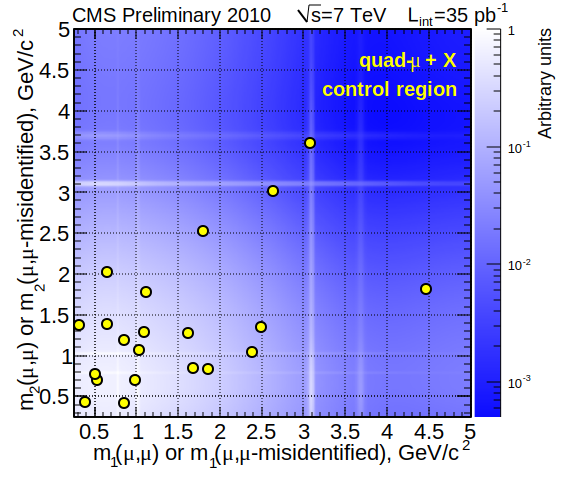
\includegraphics[width=0.35\linewidth]{PLOTS/a2_control.pdf}
\includegraphics[width=0.5\linewidth]{PLOTS/template_control__bkg_model_a2__m_1.pdf}
\caption{(a) 2D invariant mass distribution of the dimuons the $3
  \mu+$track control region for category (a-2). (b) The invariant
  masses distribution of all dimuon candidates for the same events
  (two entries per event), compared to the prediction obtained from
  the 2D background template (the sum of the $x$- and
  $y$-projections of the 2D template).\label{fig:backgroundControl_fakes}}
\end{figure}

As a second cross-check, we studied the sideband events in signal
region (a-2) by looking at the off-diagonal part of the 2-D mass
distribution. To hide a potential discovery before finalizing the
procedure, the region along the diagonal was blinded by a strip
5-$\sigma$ wide in detector resolution. Only one event is observed in
the off-diagonal region (see more details in Appendix~\ref{sec:appendix_event_displays}) consistent 
with the expectation of very low background based on a ``back of the envelope'' scaling 
$N_{4+0} = N_{3+1} \times N_{3+1}/N_{2+2} \sim 0.04\pm0.04$, which assumes that the probability 
to pick up each additional misidentified muon is roughly constant.

In a class of models with $h_{\mbox{\scriptsize dark}}\to a_{\mbox{\scriptsize dark}} a_{\mbox{\scriptsize dark}}$ where $m(h_{\mbox{\scriptsize dark}})<2m(a_{\mbox{\scriptsize dark}})$ and one or both of the $a_{\mbox{\scriptsize dark}}$ particles are off-shell, the dimuon spectrum may not show characteristic mass peaks corresponding to $m(a_{\mbox{\scriptsize dark}})$. However, in these cases one would expect a peak in the four muon invariant mass distribution. Therefore, to improve the sensitivity of this analysis to such models, we perform an additional fit of the four muon invariant mass distribution in region (a-2). The template is constructed using the same sample, two muon candidates and two tracks playing the role of misidentified muons, plotting the invariant mass of all four tracks. Figure~\ref{fig:quadmuon_background_control}(a) shows the invariant mass of such pseudo-mu-jets, which is used as a template for the background shape. Note the two-humped structure in the distribution: the second hump is due to events with two muons from a $J/\psi$ boosting the distribution for these events to higher mass. As a control region, we use the three-muon-plus-track sample with the same selections as before. The invariant mass distribution of the control region is shown in Fig.~\ref{fig:quadmuon_background_control}(b) overlaid with the background prediction using the background template fitted to the data with overall normalization being the only floating parameter. The comparison shows a good agreement, validating this technique.

\begin{figure}[tbh]
\includegraphics[width=0.5\linewidth]{PLOTS/template__bkg_model_a2_inv__m_inv.pdf}
\includegraphics[width=0.5\linewidth]{PLOTS/template_control__bkg_model_a2_inv__m_inv.pdf}
\caption{(a) Invariant mass distribution of the two pseudo-dimuon candidates in the two-muon-plus-two-tracks sample, which serves as a template for models with off-shell $a_{\mbox{\scriptsize dark}}$ in category (a-2).  (b) The same distribution for the three-muons-plus-track sample, with the background template normalization fitted to the data, showing good agreement.  \label{fig:quadmuon_background_control}}
\end{figure}

\subsection{Background Spectrum for Region (b-1)}
\label{sec:background_spectrum_for_b_1}

The (b-1) signal region consists of events with two mu-jets each
containing a single dimuon (four muons total), a signature that is
predominantly produced in the Standard Model by $b\bar{b}$ with both
$b$-quarks decaying to $\mu\mu X$. The wide mass cut used to form
mu-jets ensures that muons from nearby mu-jets do not fall in this
category and a typical background event has a topology of two
well-separated muon pairs. The fit for a possible signal in this
region is performed in the 2D space of invariant masses of the two
dimuons. Na\"ively, because each $b$-quark decays independently of the
other, the background distribution can be modeled by a Cartesian
product of two identical 1D mass templates from a $b$-jet decay,
derived from the $b\bar{b}$-enriched sample selected in
Sec.~\ref{sec:lowmassspectrum}. However, because the dimuon invariant
mass shape depends on the momentum of the $b$-quark due to momentum
cuts, care must be taken to ensure that the kinematics of the
background-enriched samples match the actual background events in the
signal region. A related consideration is that one of the dimuons
needs to contain a muon with $p_T>15$ GeV/$c$ within $|\eta|<0.9$ to
satisfy the trigger requirements, while the other dimuon does not. As
a result, the shapes of the mass spectra for the two dimuons are not
the same and must be measured separately for the ``triggered'' and
``other'' dimuons. One last consideration is a consequence of the way
the signal 2D distribution is filled when both dimuons contain a muon
satisfying trigger requirements: for these events we randomly assign
the dimuons to the triggered and other sub-classes.  This introduces a
bias in the other dimuon spectrum that needs to be included in the
modeling the background template.

To model the spectrum of the triggered dimuon, we use the
$b\bar{b}$-enriched sample selected in in
Sec.~\ref{sec:lowmassspectrum} with the $b\bar{b}$ cuts defined in
Eqn.~(\ref{eqn:bbcuts}) and require zero additional muons in the
event. These events pass minimal acceptance requirements and therefore
the dimuon always contains a trigger muon. The purity of the sample is
high (Fig.~\ref{fig:support_mass}) and we verified that these
selections do not distort the $b\bar{b}$ dimuon mass shape (more
details in the
Appendix~\ref{sec:analysis_of_the_low_mass_background_composition}). Figure~\ref{fig:backgroundEnriched_massCF}
shows the invariant mass distribution of the triggered dimuons and the
parameterized function fitted to the data, which will be used to
construct the 2D template. The parameterized template uses the same
universal functional form from Eqn.~(\ref{eqn:bkg_shape}) with some of
the parameters fixed.

To model the kinematics of the ``other'' dimuon, we use the $b\bar{b}$-enriched
sample to select events containing a dimuon (not required to contain a
trigger-quality muon) and one additional muon: the additional muon is
required to satisfy the trigger.  Three-muon events with a small angle
between two of the muons are predominantly $b\bar{b}$ with one
$b$-quark decaying to $\mu\mu X$ and the other to $\mu Y$. These
selections ensure that the dimuon is unbiased by the trigger and also
has approximately the same kinematics as the events entering the
signal region. Finally, we plot the invariant mass of selected dimuons
with a weighting factor of $\tfrac{1}{2}$ to dimuons that contain a
trigger-quality muon. This additional weighting is necessary to
account for the bias in constructing the signal region 2D distribution
for events with two trigger dimuons.  (See
Appendix~\ref{sec:appendix_b_1_weighting}
for details.) The resultant distribution for the other
dimuon, along with the parameterized template to be used in the 2D
mass template for the final fit, is shown in
Fig.~\ref{fig:backgroundEnriched_massCF}(b).

\begin{figure}
\centering
\includegraphics[width=0.45\linewidth]{PLOTS/template__bg_sh_b1t__m_1_log.pdf}
\includegraphics[width=0.45\linewidth]{PLOTS/template__bg_sh_b1o__m_2_log.pdf}
\includegraphics[width=0.45\linewidth]{PLOTS/template_control__bkg_model_b1.pdf}
\caption{(a): dimuons with $b\bar{b}$ cuts (background-enriched
  region for triggered dimuon in (b-1)). (b): dimuons plus
  additional, triggered muon (background-enriched region for other
  dimuon in (b-1)). (c): The distribution of all dimuons in the off-diagonal part
 of the distribution in (b-1) compared to the prediction for the background shape 
 obtained from the full 2D template and fitted to data for overall normalization only.  \label{fig:backgroundEnriched_massCF}}
\end{figure}

The final 2D background template is built from a Cartesian product of
two parameterized 1D shapes for the triggered and other dimuons. As a
cross-check, we compared the constructed background templates for both
the triggered and other dimuons in signal region (b-1) with the
background predictions using simulation.  A large sample of $b\bar{b}
\to 2\mu \, 2\mu \, X$ Monte Carlo, simulated by Pythia 6 and decayed
by EvtGen, was used to select events passing all region (b-1)
selections. We verified that the 2D distribution has no correlations
between the masses of the two dimuons, confirming the assumption used
in constructing the background template that the 2D distribution is
factorizable. In addition, the final background distributions for the
triggered and other dimuons were compared with the data-driven
templates, showing reasonably good agreement (see
Appendix~\ref{sec:appendix_factorizable_b_1}).

To validate the technique, we use events satisfying selections for the
(b-1) signal region, but in the off-diagonal part of the dimuon-dimuon
mass plane (a 5-$\sigma$ strip along the diagonal was blinded). Ten
events were observed in that region, consistent with
back-of-the-envelope scaling of the $b\bar{b} \to 2\mu X$ sample:
$N_{4\mu+X} \sim \tfrac{1}{2} N_{2\mu+X} \mathcal{B}(b \to 2\mu
X) = \tfrac{1}{2} \times 12\,841 \times 0.002 = 12.8$ events. The distribution 
of these events is consistent with the background template, as shown in 
Fig.~\ref{fig:backgroundEnriched_massCF}(c).
